%%%
%
% $Autor: Wings $
% $Datum: 2021-05-14 $
% $Pfad: GitLab/MLEdgeComputer $
% $Dateiname: SydeCloud
% $Version: 4620 $
%
% !TeX spellcheck = de_DE/GB
% !TeX program = pdflatex
% !BIB program = biber/bibtex
% !TeX encoding = utf8
%
%%%



\chapter{Syde Cloud}

\section{Access}

\URL{https://syde.cloud}

\bigskip

\begin{tabular}{ll}
    User:     & \textcolor{blue}{WingsESSCloud@gmail.com} \\
    password: & Fibo.1.1.2.3.5.8.13 \\
\end{tabular}


\section{Usage}

\begin{center}
    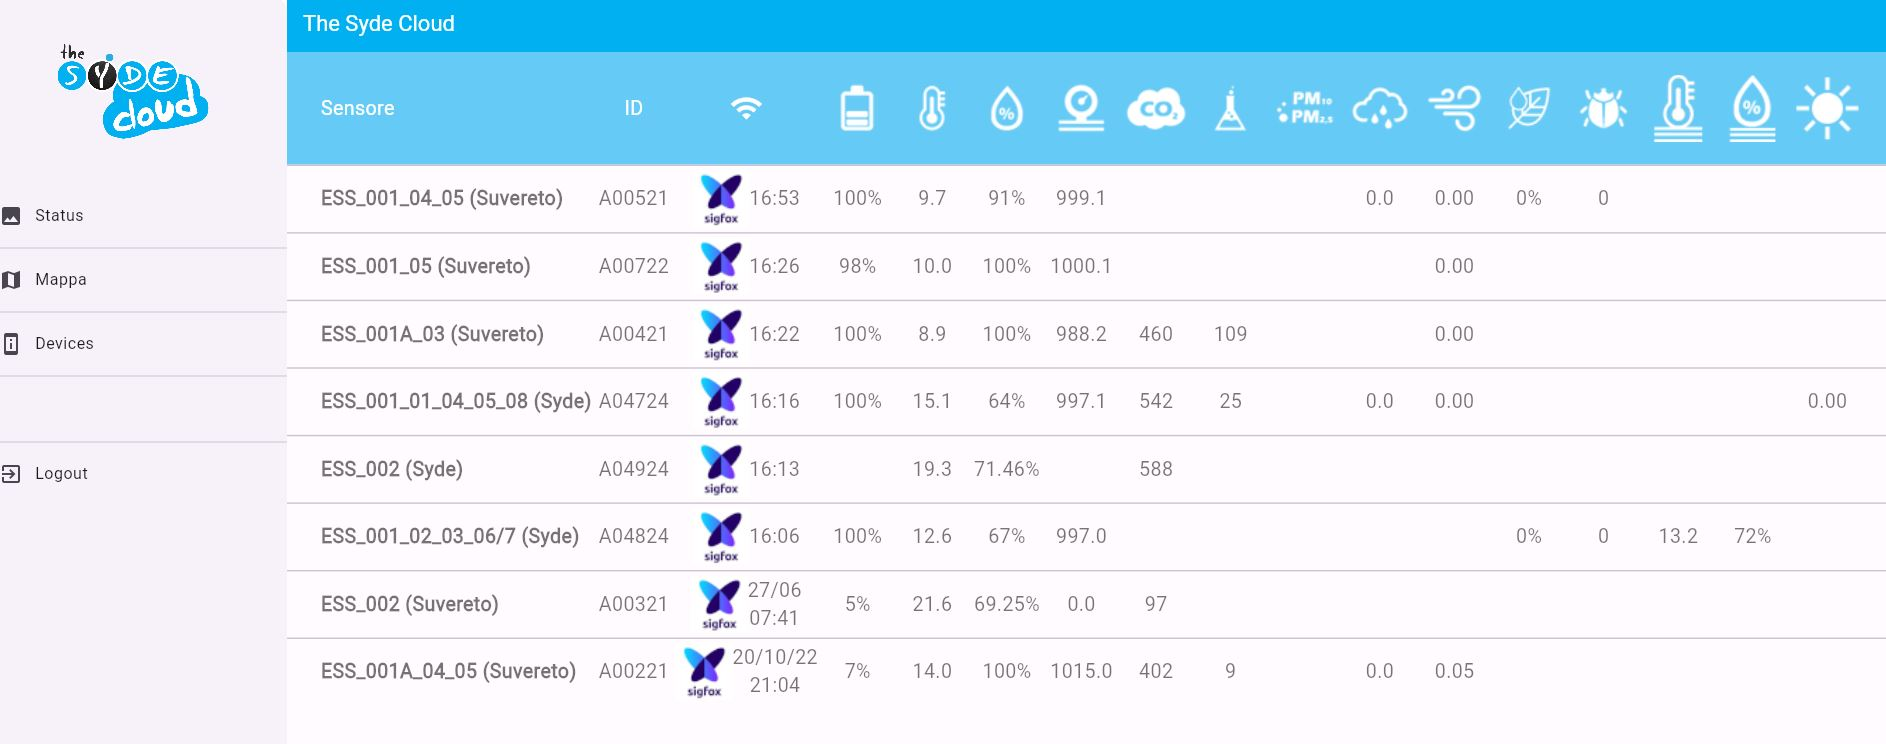
\includegraphics[width=\textwidth]{../../Images/Syde/SydeCloud}
    \captionof{figure}{View of the Syde Cloud after access}
\end{center}

\bigskip

If you click on one value, then you get the values of the sensor of the last month.

\begin{center}
    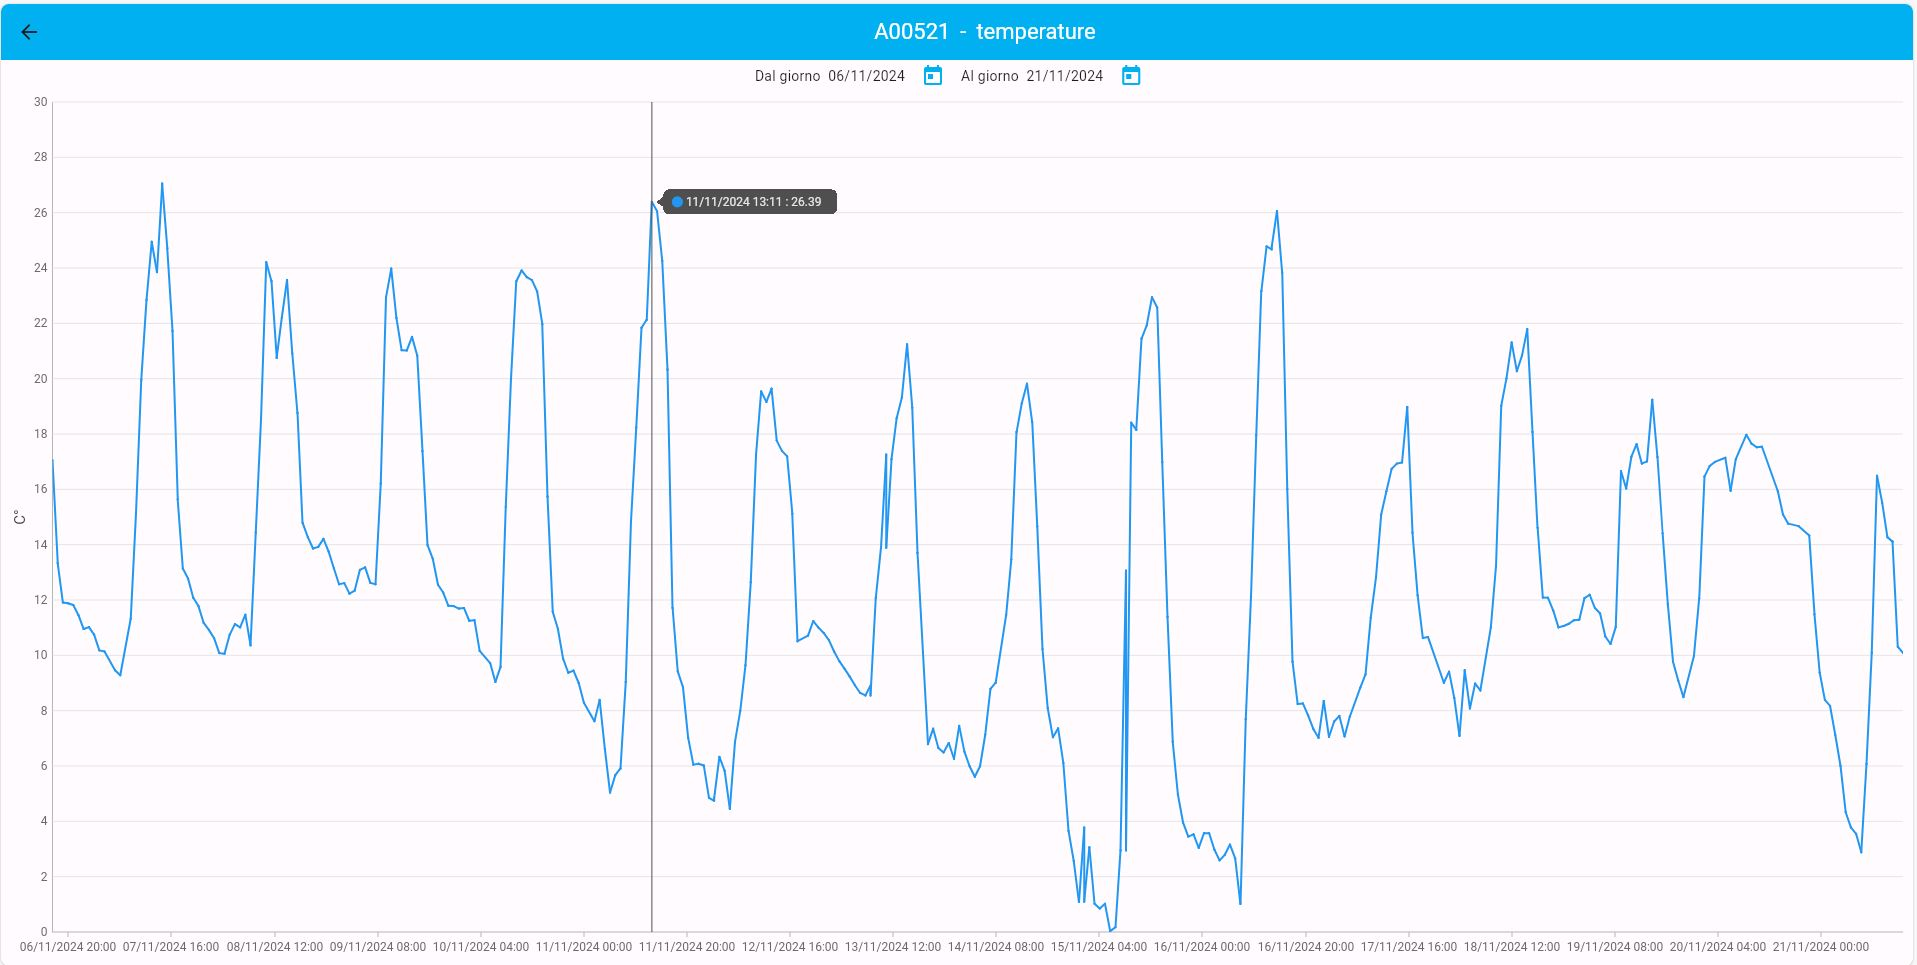
\includegraphics[width=\textwidth]{../../Images/Syde/SydeCloudSensorTemperature}
    \captionof{figure}{Values of the temperature sensor A00521 of the last two weeks.}
\end{center}



\section{Data}

You can connect some sensors to the system. But not everytime all sensors are connected. Now, we list all possible sensors which are shown in the Syde Cloud.

\subsection{Sensor's Name}

Symbol: \quad 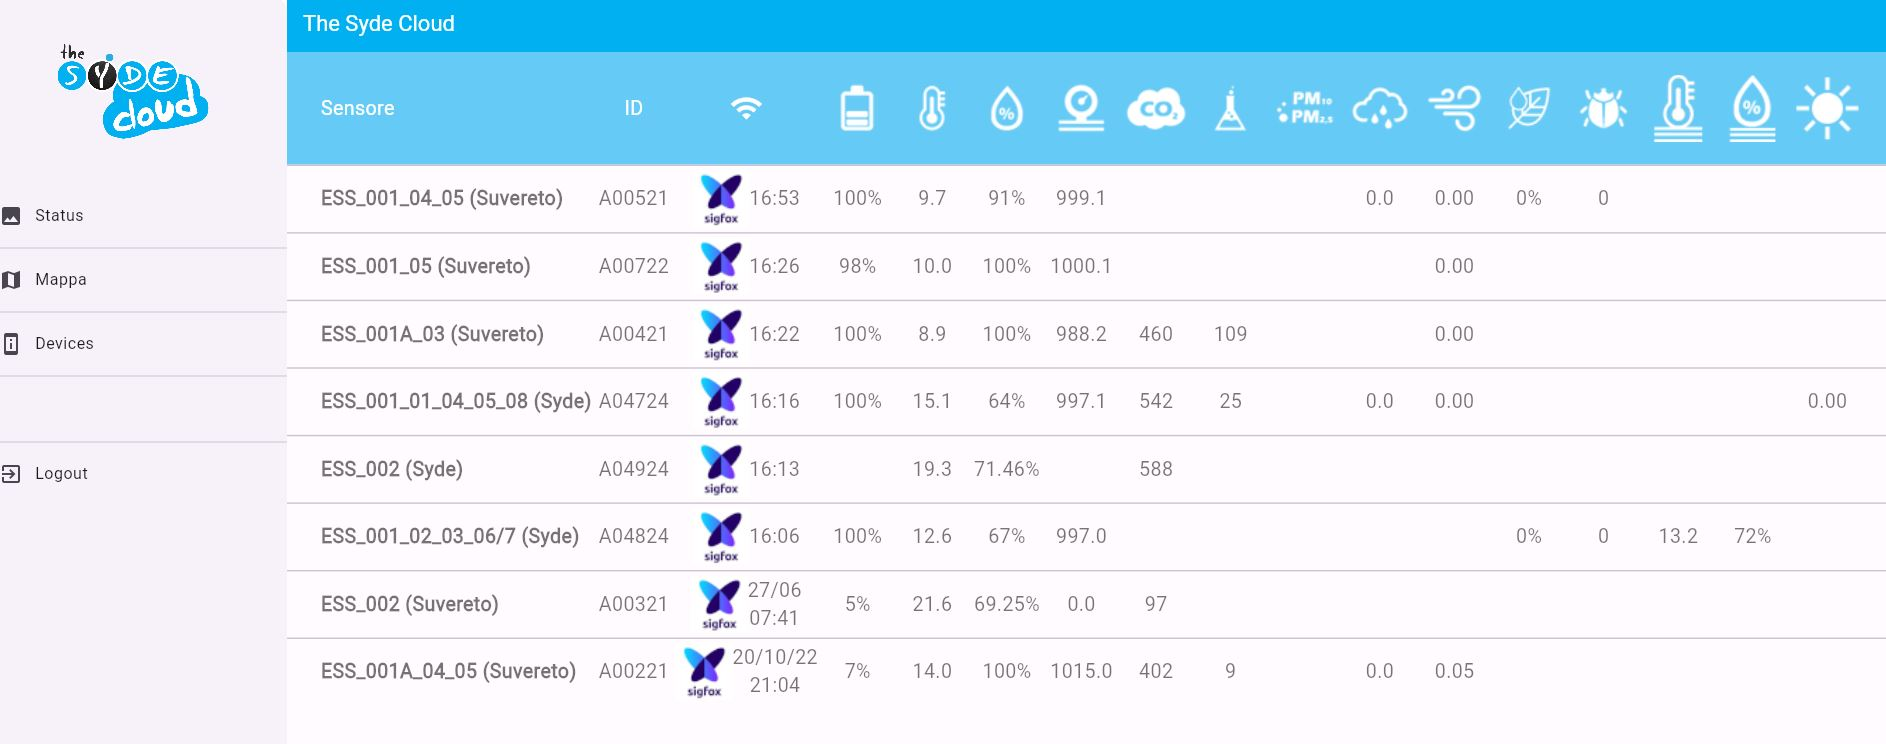
\includegraphics[trim=40mm 80mm 194mm 10mm, clip,scale=0.5]{../../Images/Syde/SydeCloud}

\bigskip

description: Name of the sensor, e.g. ESS\_001\_01\_04\_05\_08 (Syde)


\bigskip

Unit: ./.

\bigskip

Minimum: ./.

\bigskip

Maximum: ./.


\subsection{Sensor Identification}

Symbol: \quad 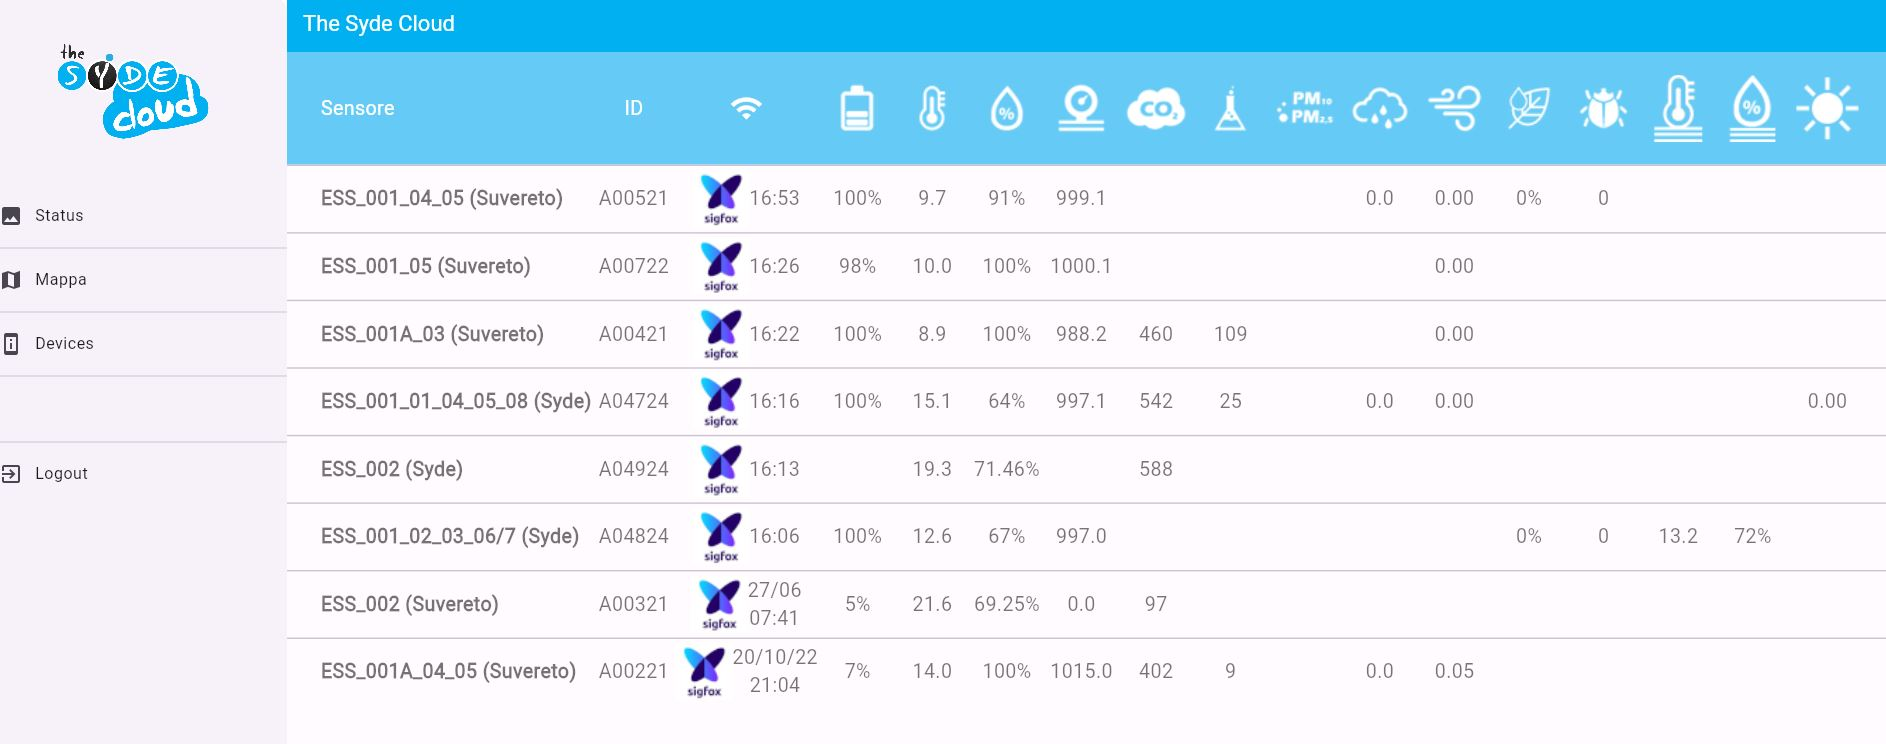
\includegraphics[trim=80mm 80mm 161mm 10mm, clip,scale=0.5]{../../Images/Syde/SydeCloud}

\bigskip

description: Unique number of the sensor, e.g. A04724


\bigskip

Unit: ./.

\bigskip

Minimum: ./.

\bigskip

Maximum: ./.


\subsection{Connection}

Symbol: \quad 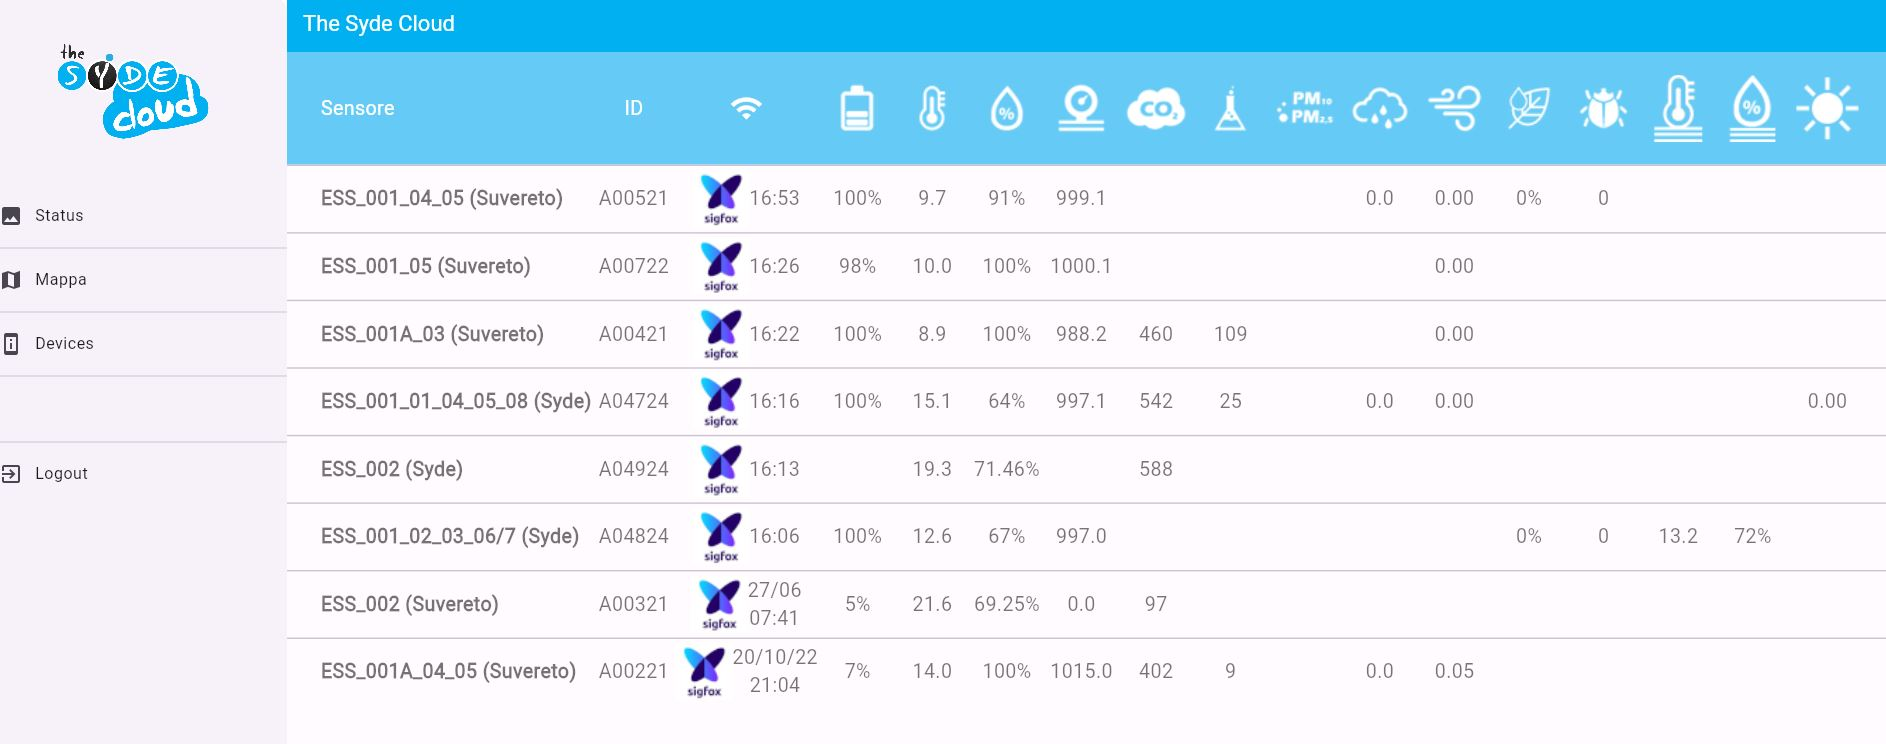
\includegraphics[trim=95mm 80mm 147mm 10mm, clip,scale=0.5]{../../Images/Syde/SydeCloud}


\bigskip

description: Symbol of the protocol, e.g. via sigfox  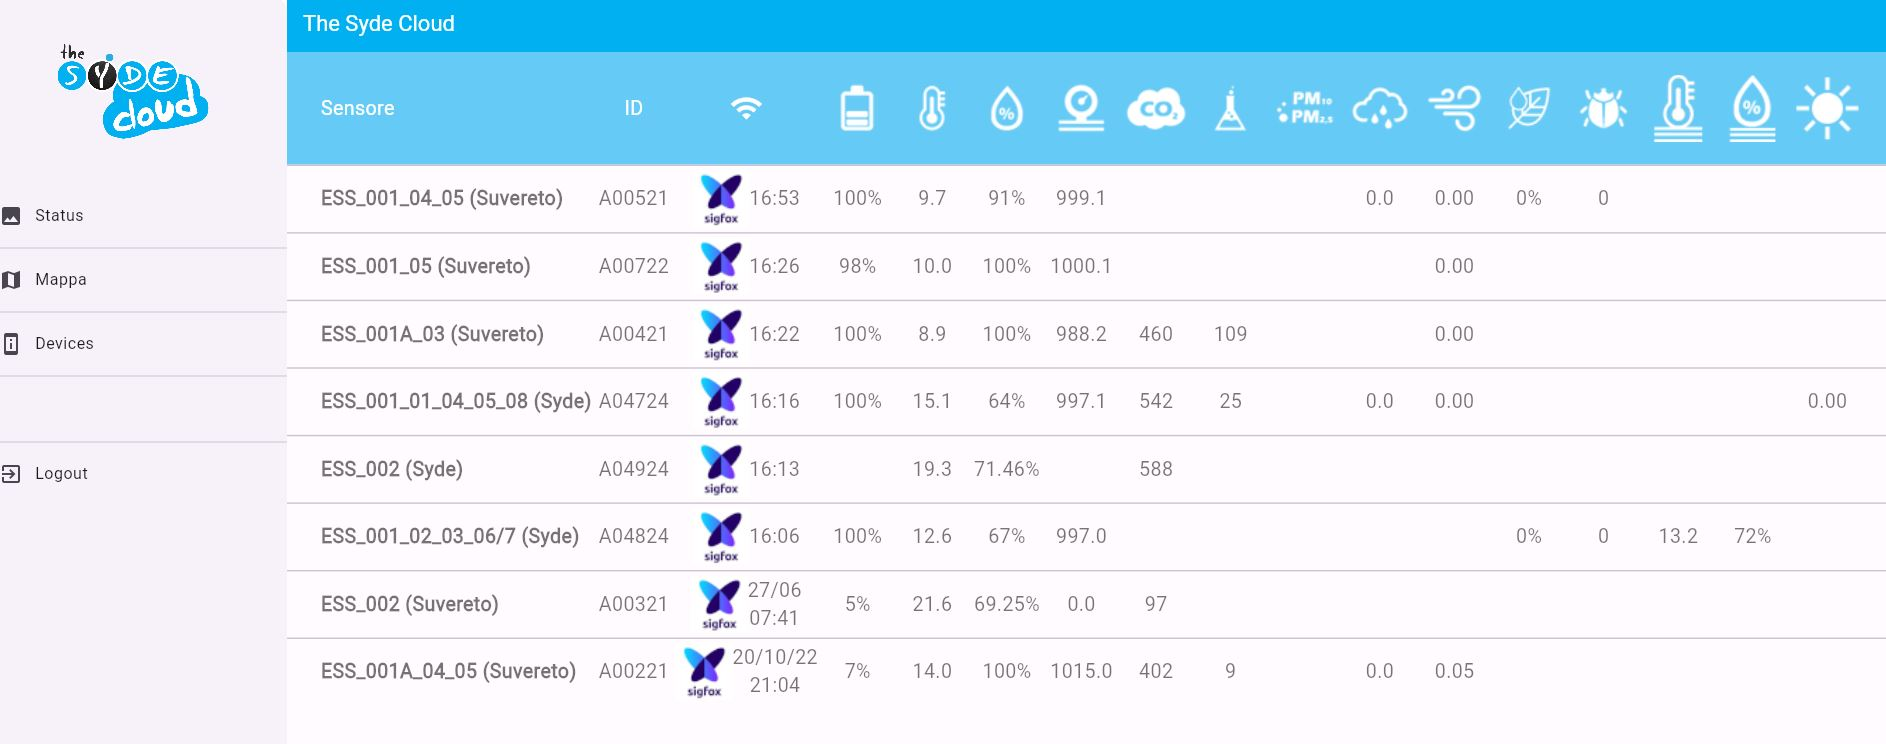
\includegraphics[trim=92mm 50mm 150mm 40mm, clip,scale=0.6]{../../Images/Syde/SydeCloud}


It is coded inside the sensor's name. 


\bigskip

Unit: ./.

\bigskip

Minimum: ./.

\bigskip

Maximum: ./.


\subsection{State of Charge of the Battery}

Symbol: \quad 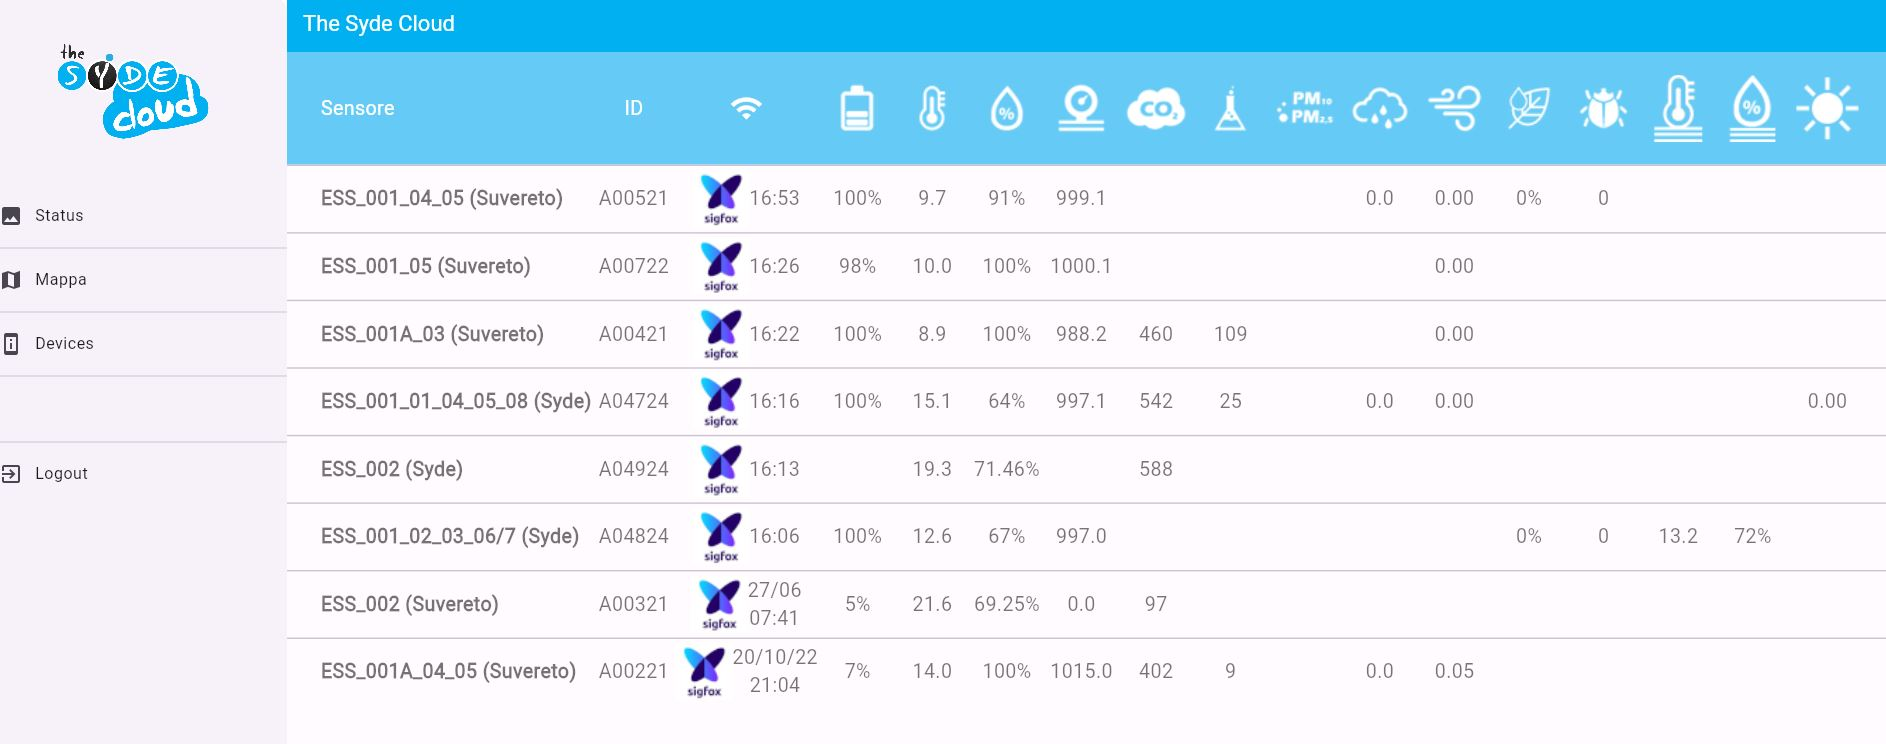
\includegraphics[trim=108mm 80mm 130mm 10mm, clip,scale=0.5]{../../Images/Syde/SydeCloud}


\bigskip

description: State of charge of the battery


\bigskip

Unit: \%

\bigskip

Minimum: 0 

\bigskip

Maximum: 100 

\subsection{Air Temperature}

Symbol: \quad 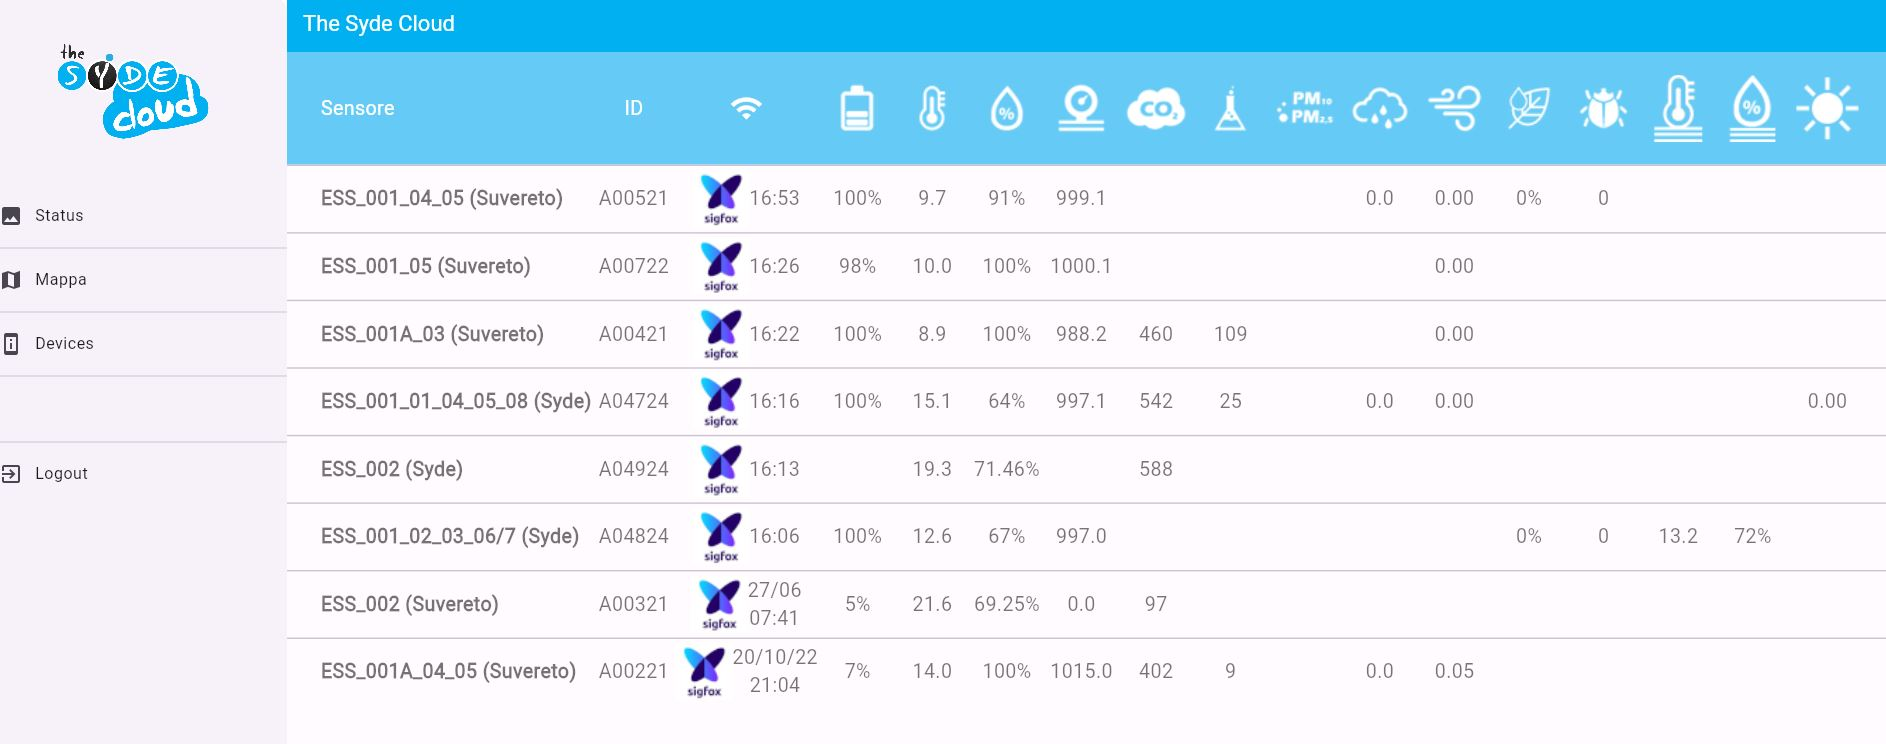
\includegraphics[trim=120mm 80mm 122.5mm 10mm, clip,scale=0.5]{../../Images/Syde/SydeCloud}


\bigskip

description: Air temperature



\bigskip

Unit: Celsius $^\circ$ 

\bigskip

Minimum: It depends on the sensor; e.g. -40  

\bigskip

Maximum: It depends on the sensor; e.g. 85


\subsection{Air Humidity}

Symbol: \quad 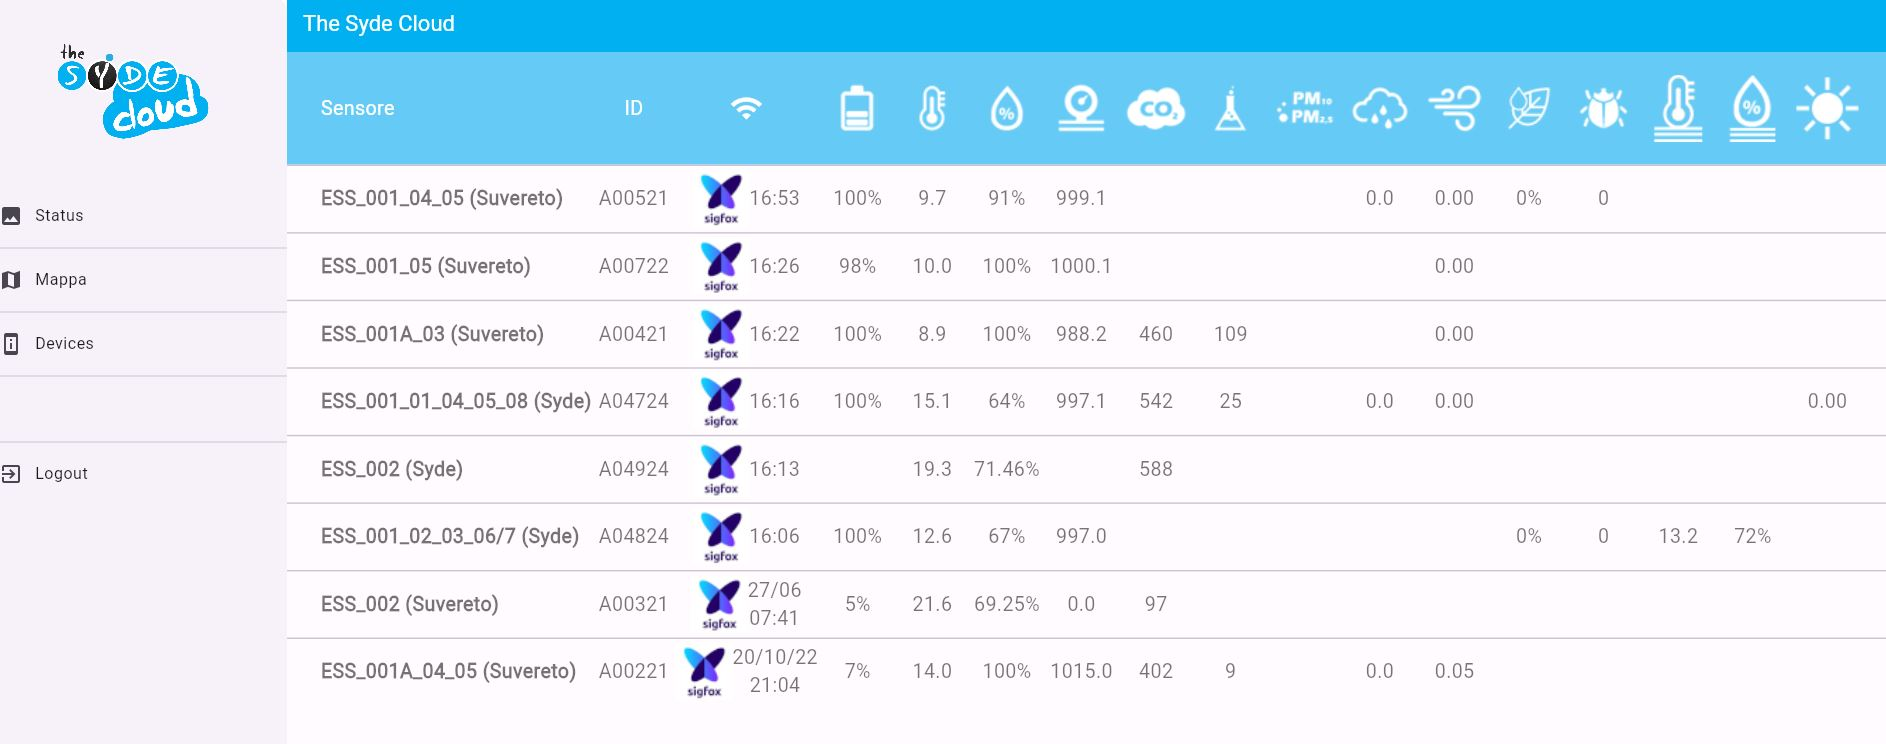
\includegraphics[trim=129mm 80mm 113mm 10mm, clip,scale=0.5]{../../Images/Syde/SydeCloud}


\bigskip

description: Air humidity



\bigskip

Unit: \%

\bigskip

Minimum: 0 

\bigskip

Maximum: 100 


\subsection{Air Pressure}

Symbol: \quad 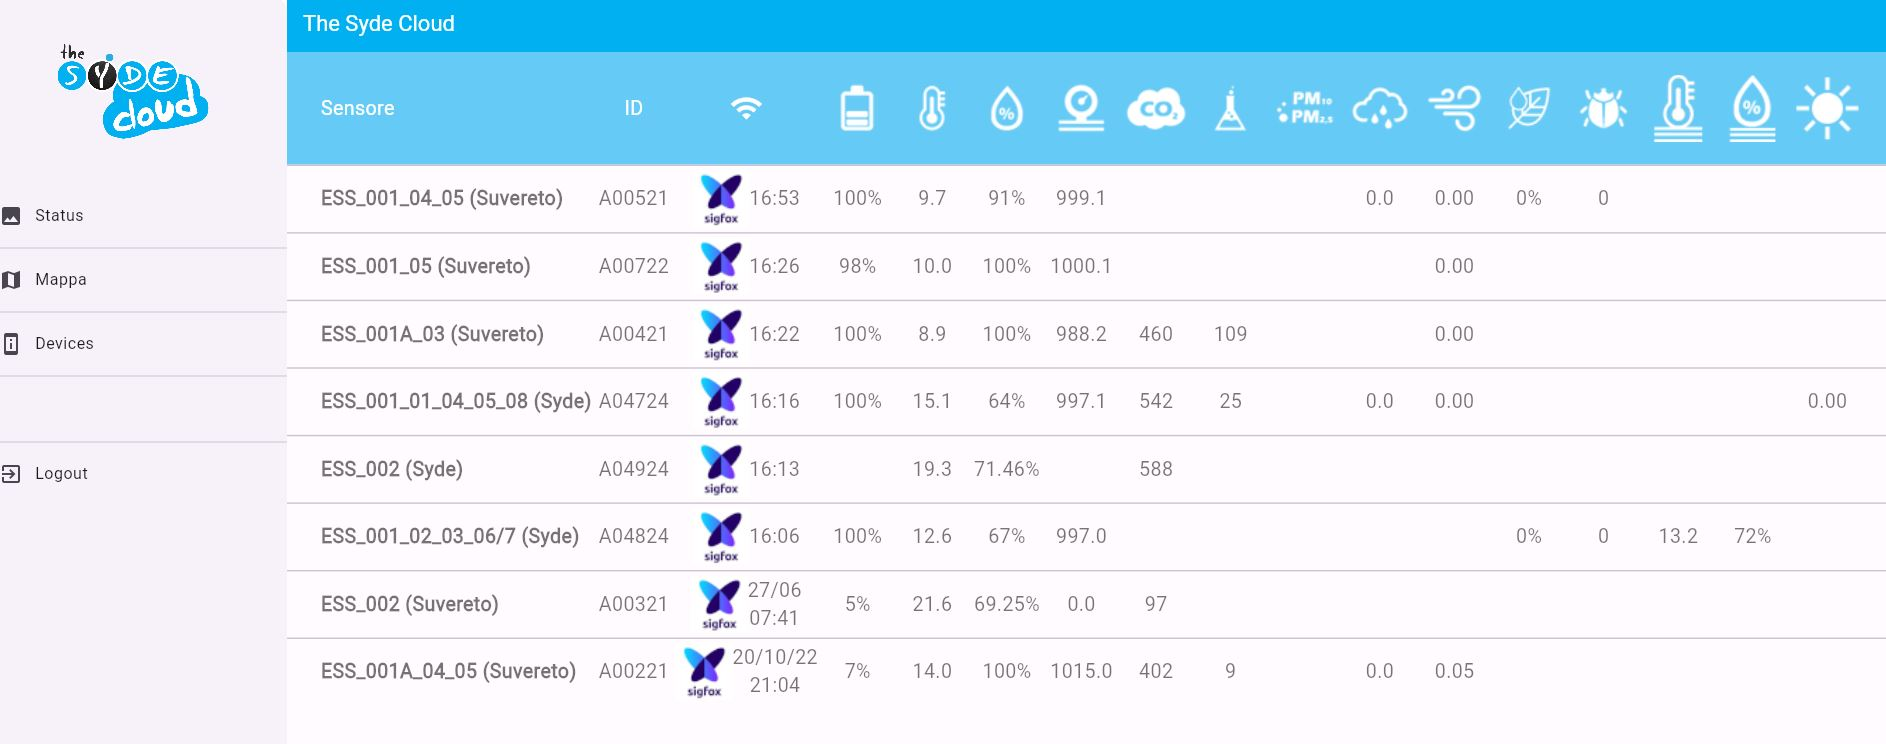
\includegraphics[trim=138mm 80mm 101mm 10mm, clip,scale=0.5]{../../Images/Syde/SydeCloud}


\bigskip

Description: Air pressure



\bigskip

Unit: hPa

\bigskip

Minimum: 300

\bigskip

Maximum: 1100


\subsection{Carbon Dioxide}

Symbol: \quad 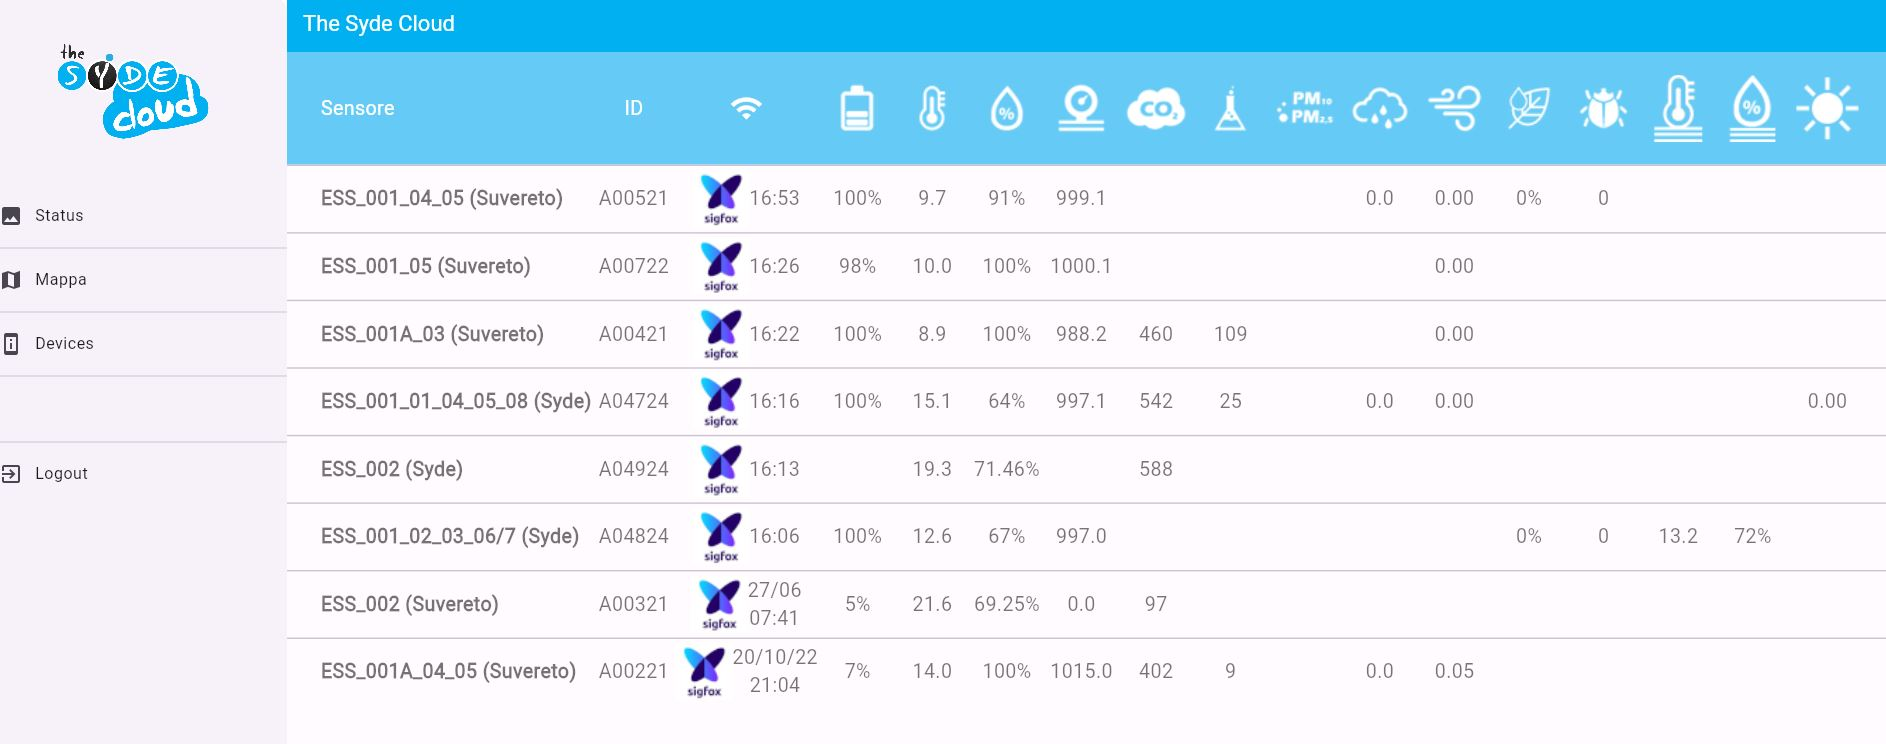
\includegraphics[trim=149mm 80mm 92mm 10mm, clip,scale=0.5]{../../Images/Syde/SydeCloud}


\bigskip

description: Carbon dioxide in the air



\bigskip

Unit: ppm

\bigskip

Minimum: 0

\bigskip

Maximum: 1500

\subsection{Volatile Organic Compound}

Symbol: \quad 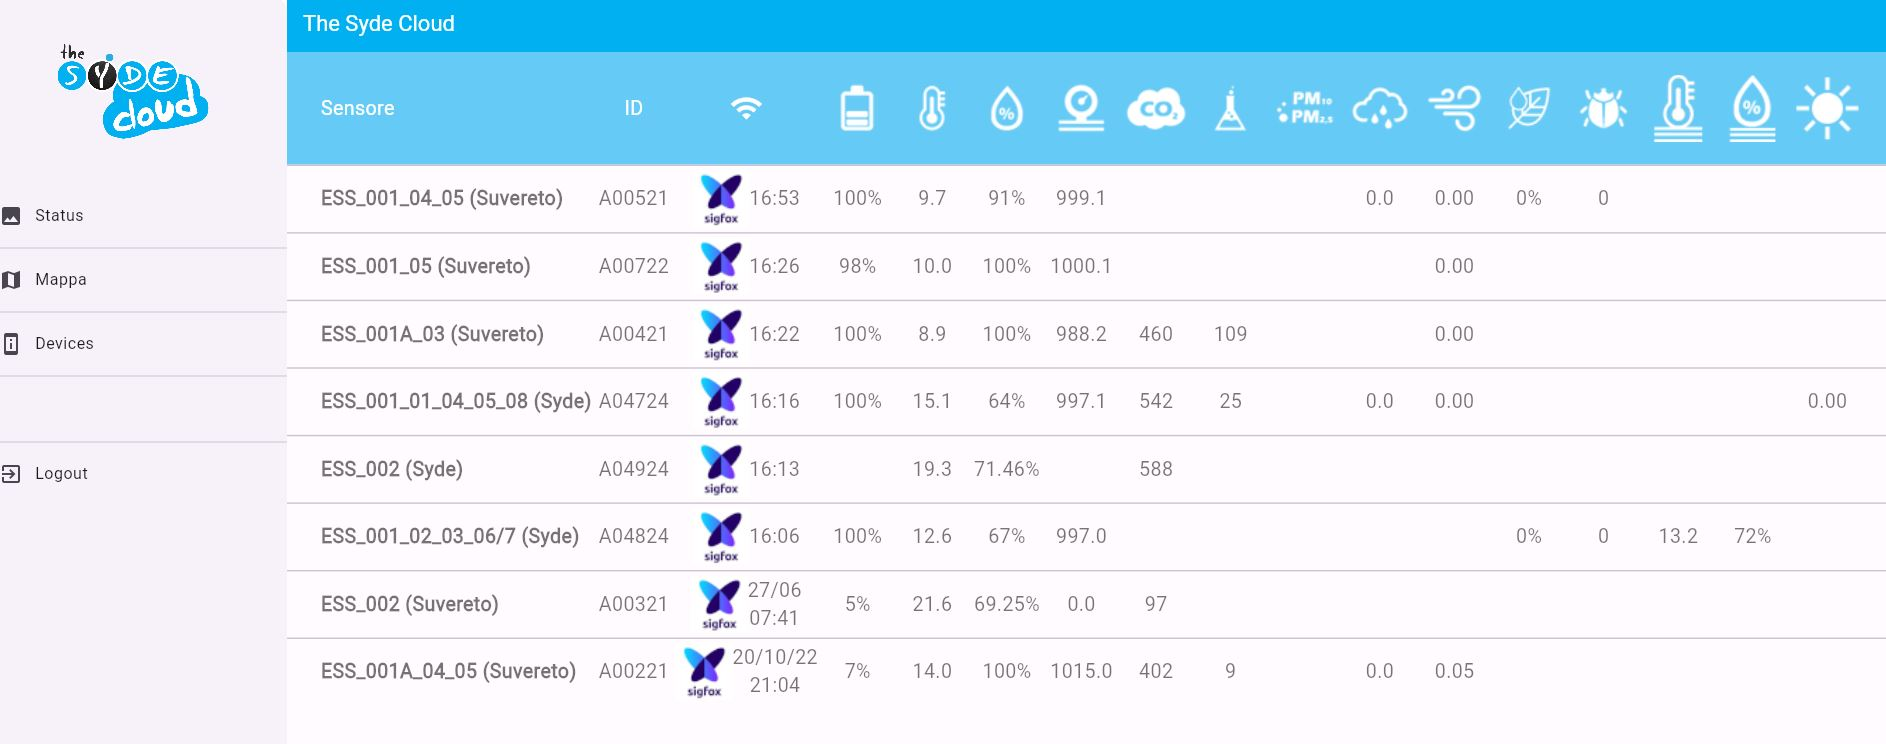
\includegraphics[trim=158.5mm 80mm 83mm 10mm, clip,scale=0.5]{../../Images/Syde/SydeCloud}


\bigskip

Description: Volatile organic compound

%\url{https://en.wikipedia.org/wiki/Volatile_organic_compound}


\bigskip

Unit: ppm

\bigskip

Minimum: 0 

\bigskip

Maximum: 60,000


\subsection{Particulates}

Symbol: \quad 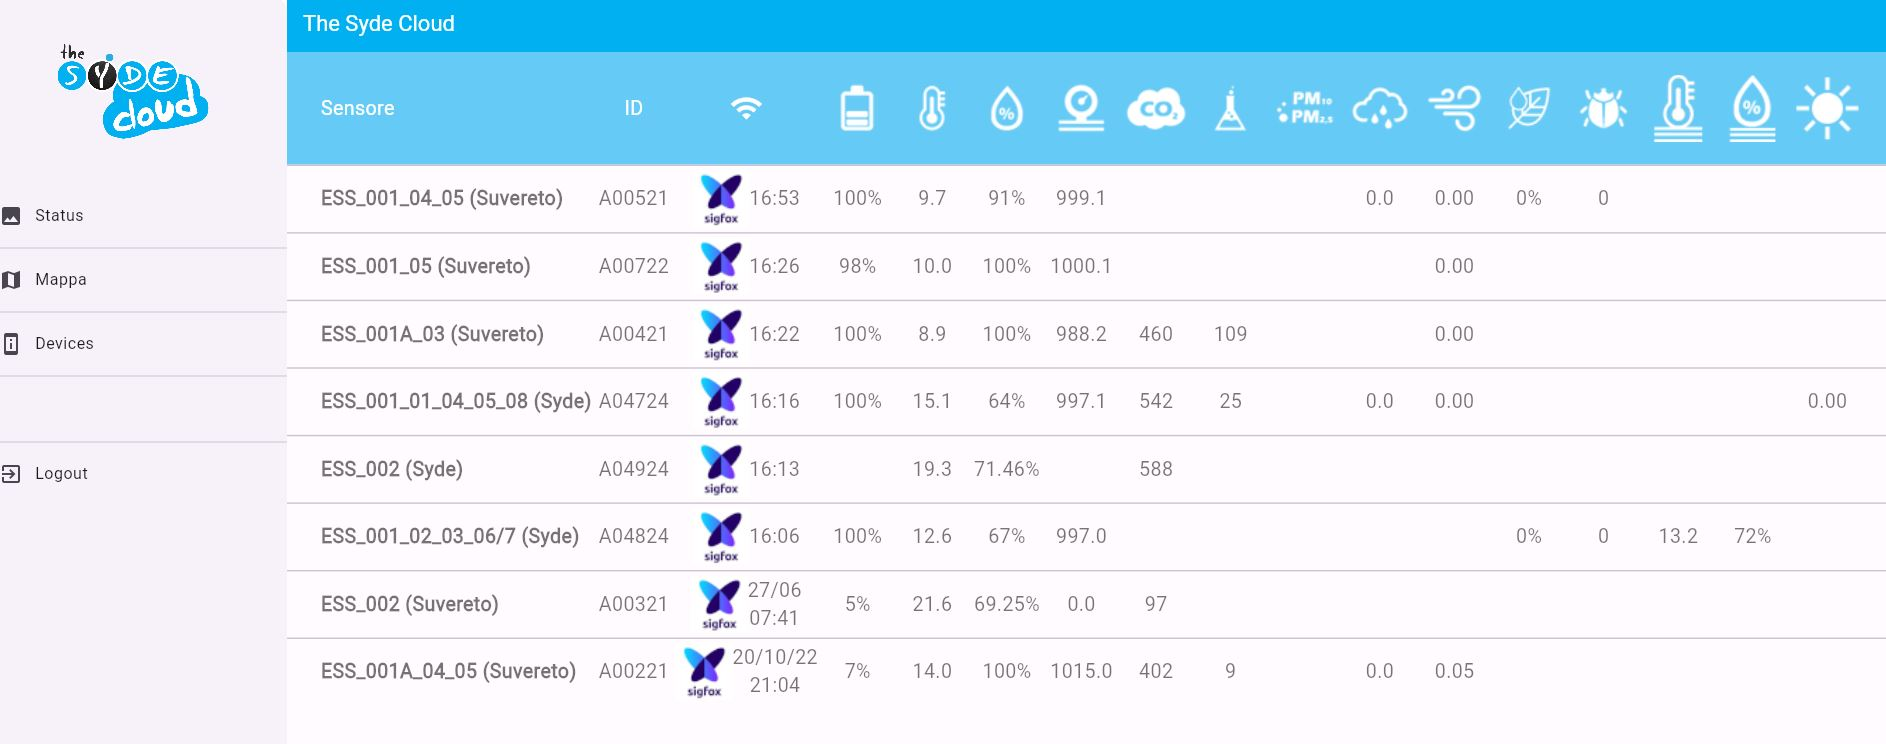
\includegraphics[trim=167mm 80mm 72mm 10mm, clip,scale=0.5]{../../Images/Syde/SydeCloud}

\bigskip

Description: Particulates in the air

\bigskip

Unit: ppm

\bigskip

Minimum: 0 

\bigskip

Maximum: 50,000 


\subsection{Precipitation}

Symbol: \quad 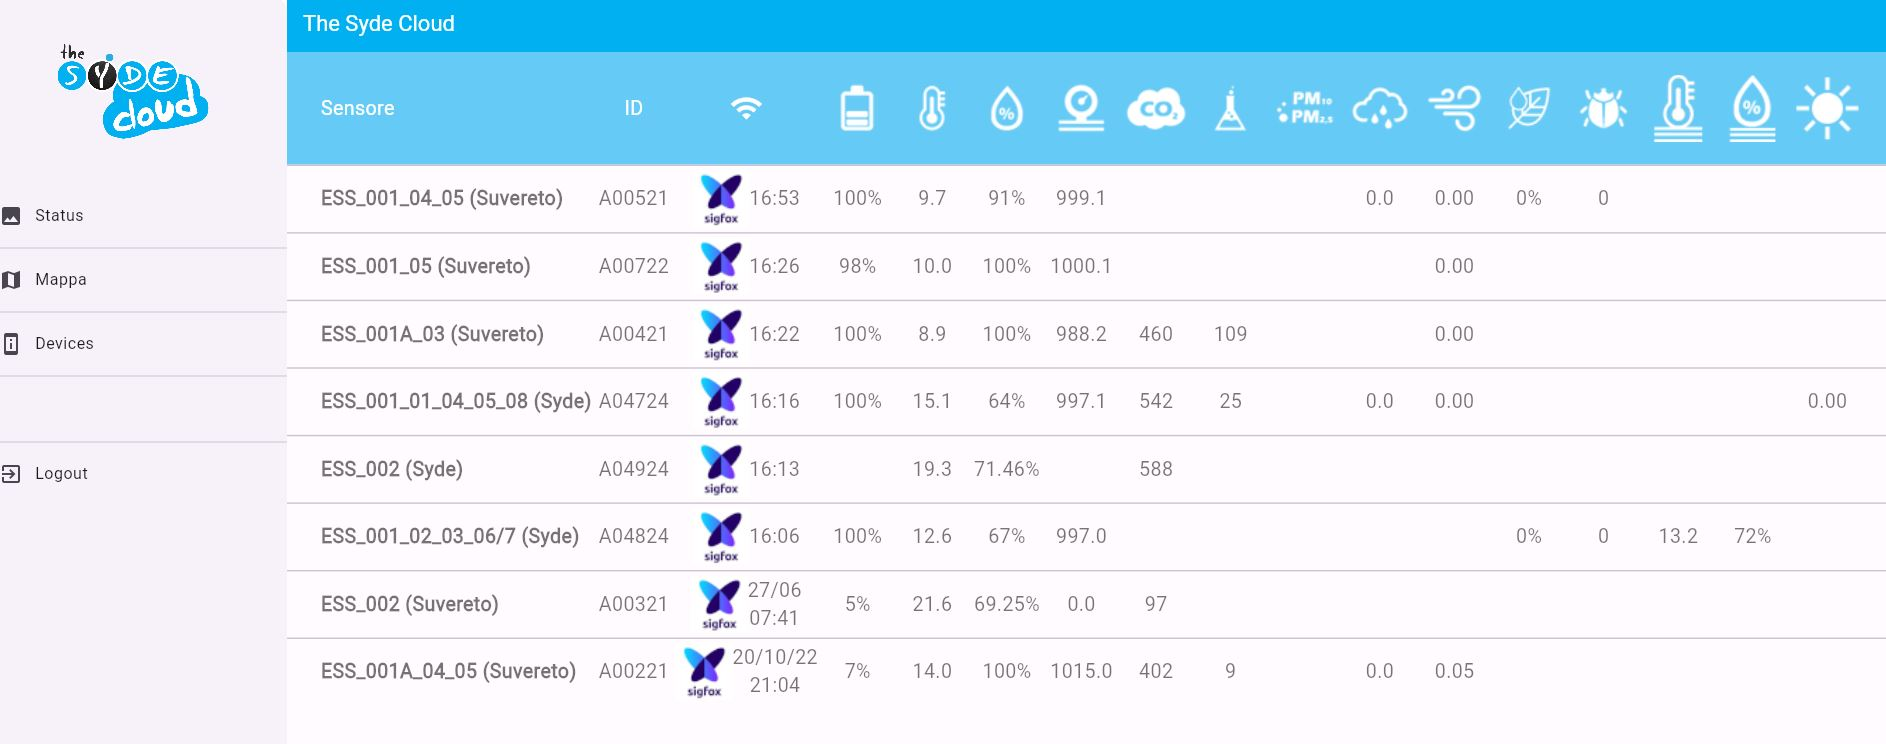
\includegraphics[trim=177mm 80mm 62mm 10mm, clip,scale=0.5]{../../Images/Syde/SydeCloud}


\bigskip

Description: Precipitation

\medskip

Resolution: 0.5

\bigskip

Unit: mm

\bigskip

Minimum: 0.5 

\bigskip

Maximum: 100,000 


\subsection{Wind Speed}

Symbol: \quad 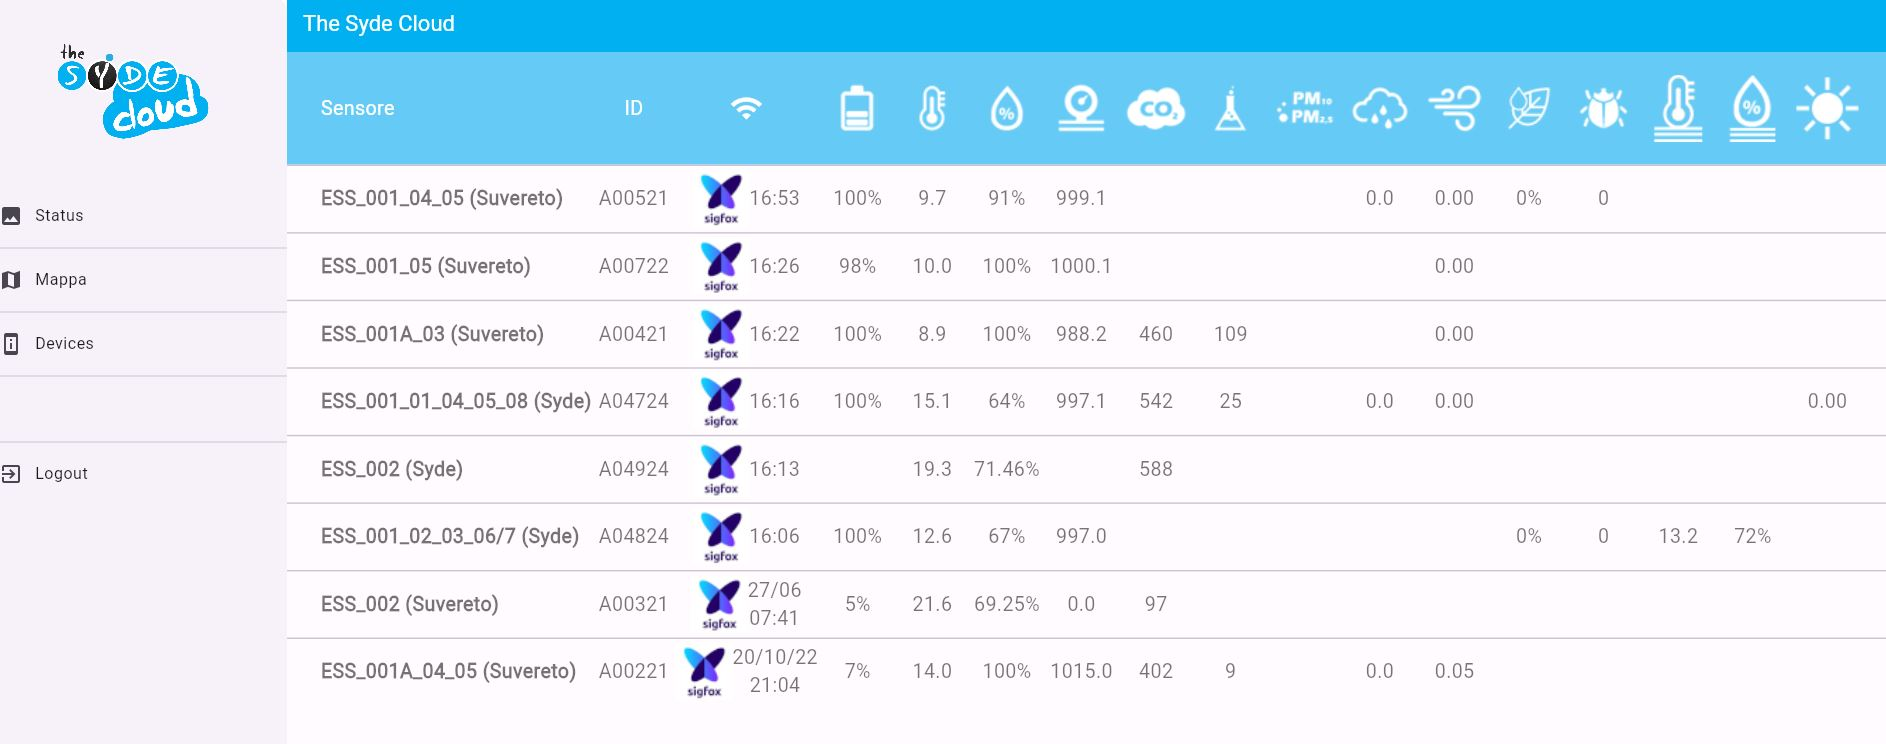
\includegraphics[trim=188mm 80mm 52mm 10mm, clip,scale=0.5]{../../Images/Syde/SydeCloud}


\bigskip

Description: Wind speed



\bigskip

Unit: $\frac{m}{s}$

\bigskip

Minimum: 0.1

\bigskip

Maximum: 100,000 


\subsection{Moisture on the Leaves}

Symbol: \quad 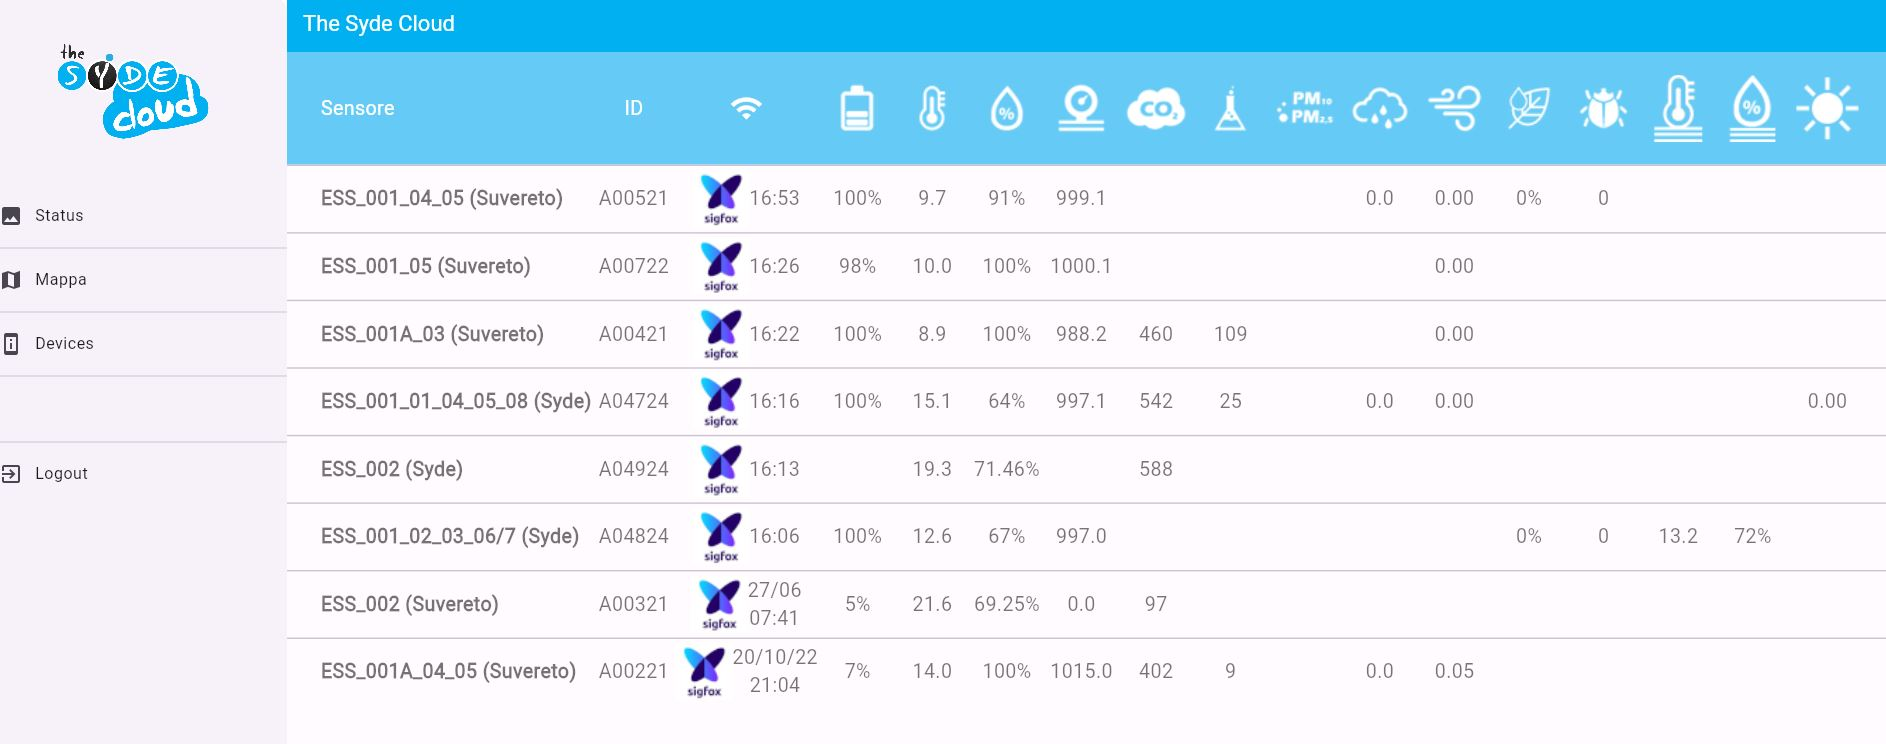
\includegraphics[trim=198mm 80mm 42mm 10mm, clip,scale=0.5]{../../Images/Syde/SydeCloud}


\bigskip

Description: Moisture on the Leaves



\bigskip

Unit: \%
%pF

\bigskip

Minimum: 0 

\bigskip

Maximum: 100


\subsection{Parasites}


Symbol: \quad 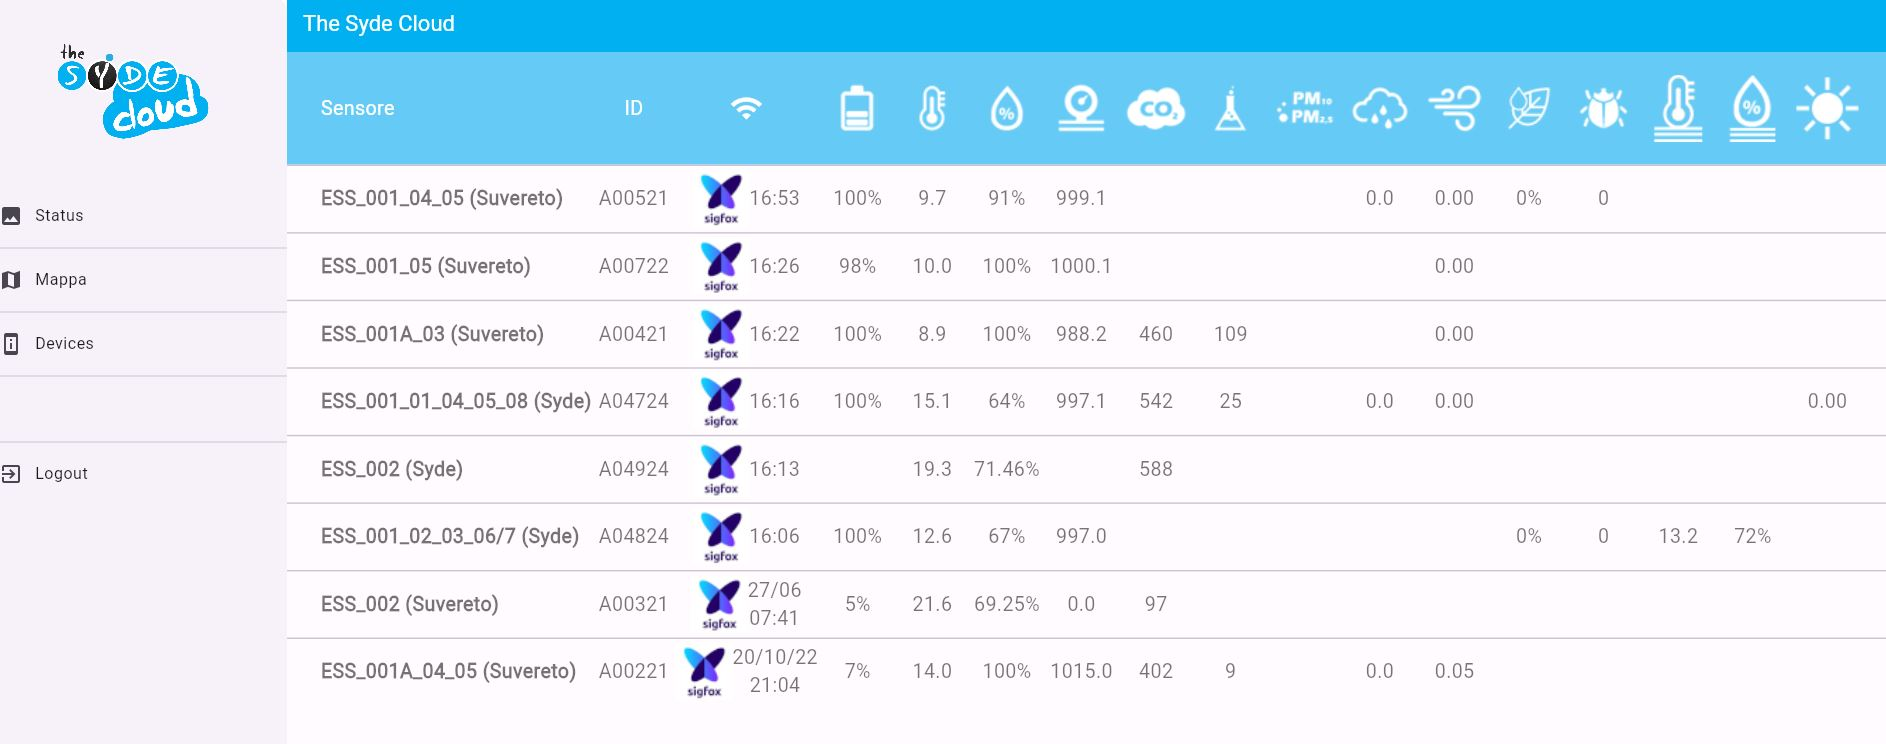
\includegraphics[trim=208mm 80mm 32.6mm 10mm, clip,scale=0.5]{../../Images/Syde/SydeCloud}


\bigskip

Description: Number of parasites in the trap

\bigskip

Unit: ./. (Counter)

\bigskip

Minimum: 0 

\bigskip

Maximum: 100,000


\subsection{Soil Temperature}

Symbol: \quad 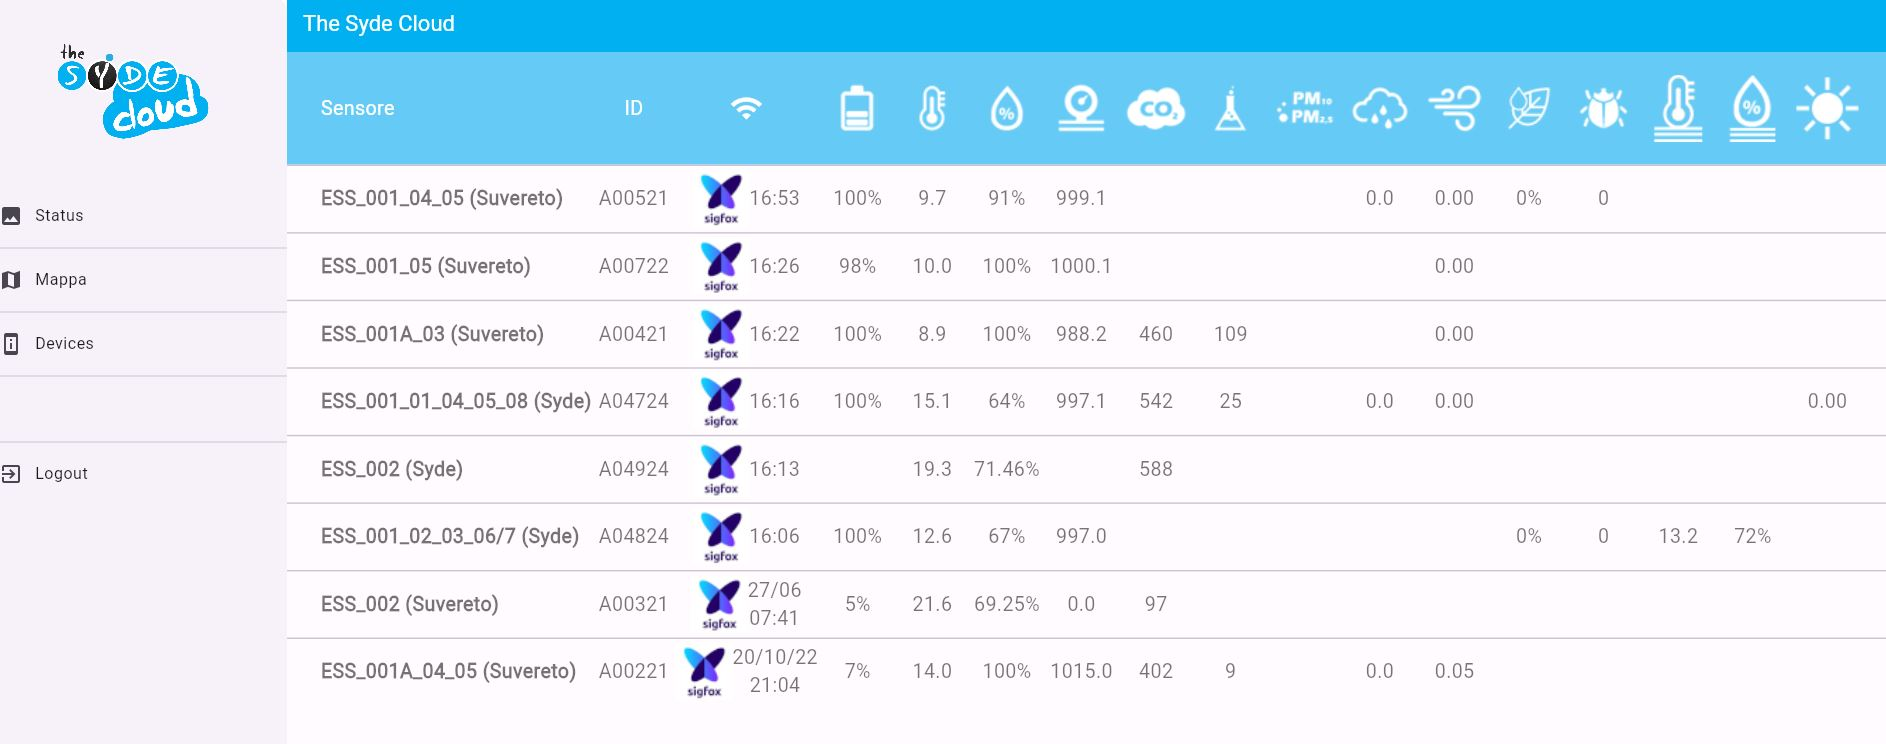
\includegraphics[trim=218mm 80mm 22.5mm 10mm, clip,scale=0.5]{../../Images/Syde/SydeCloud}


\bigskip

Description: Soil temperature



\bigskip

Unit: $^\circ$ Celsius

\bigskip

Minimum: -40

\bigskip

Maximum: 85 

\subsection{Soil Moisture}

Symbol: \quad 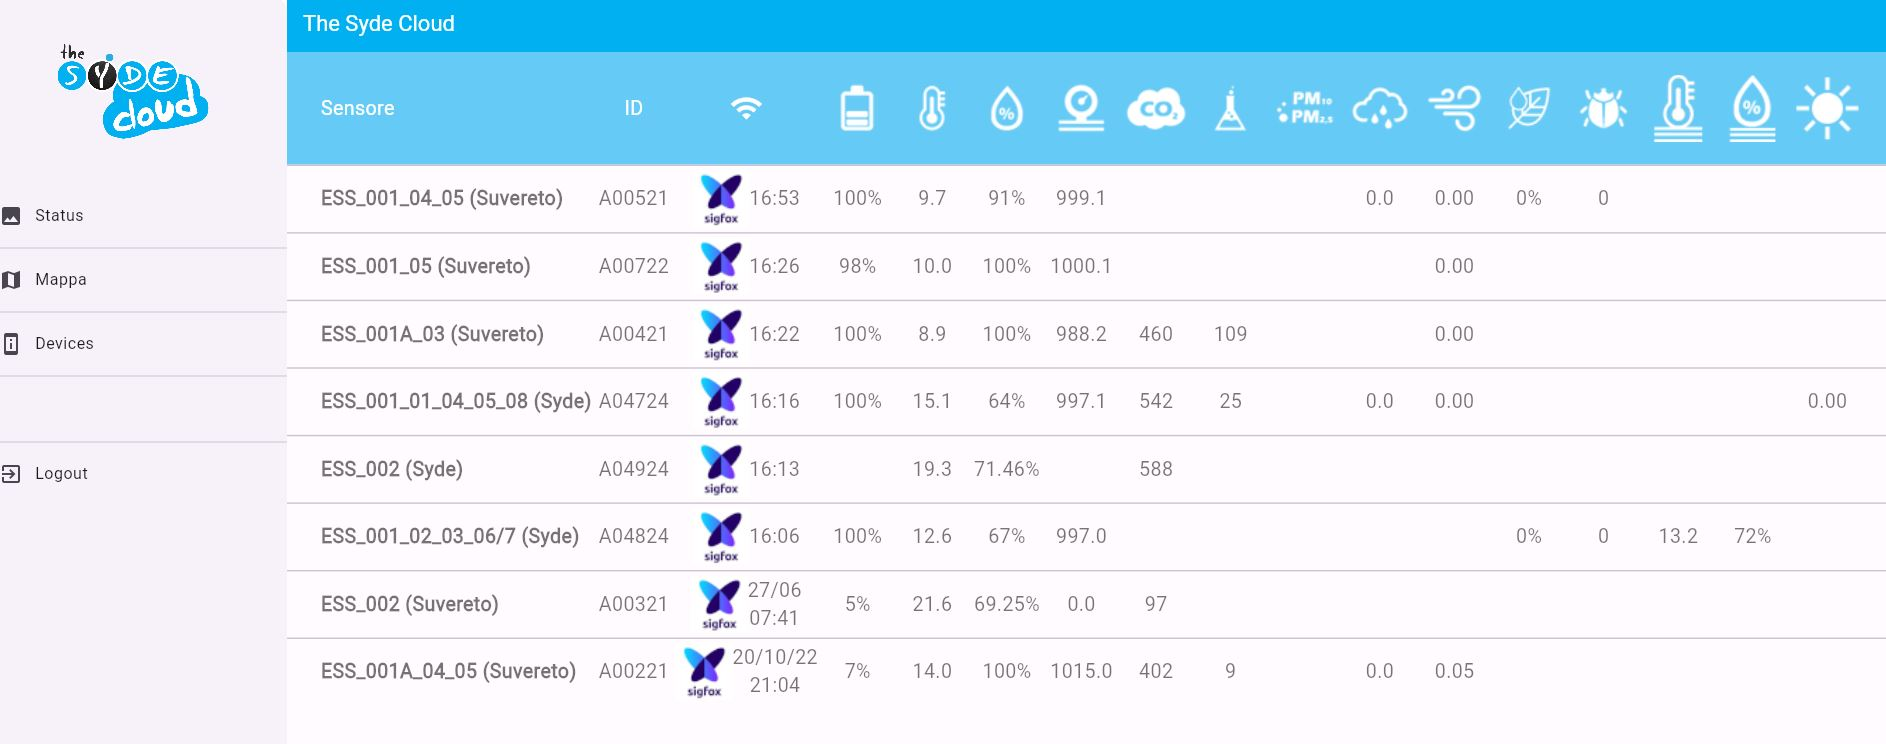
\includegraphics[trim=227.1mm 80mm 12.5mm 10mm, clip,scale=0.5]{../../Images/Syde/SydeCloud}


\bigskip

Description: Soil moisture



\bigskip

Unit: \%

\bigskip

Minimum: 0 \%

\bigskip

Maximum: 100 \%


\subsection{Brightness}

Symbol: \quad 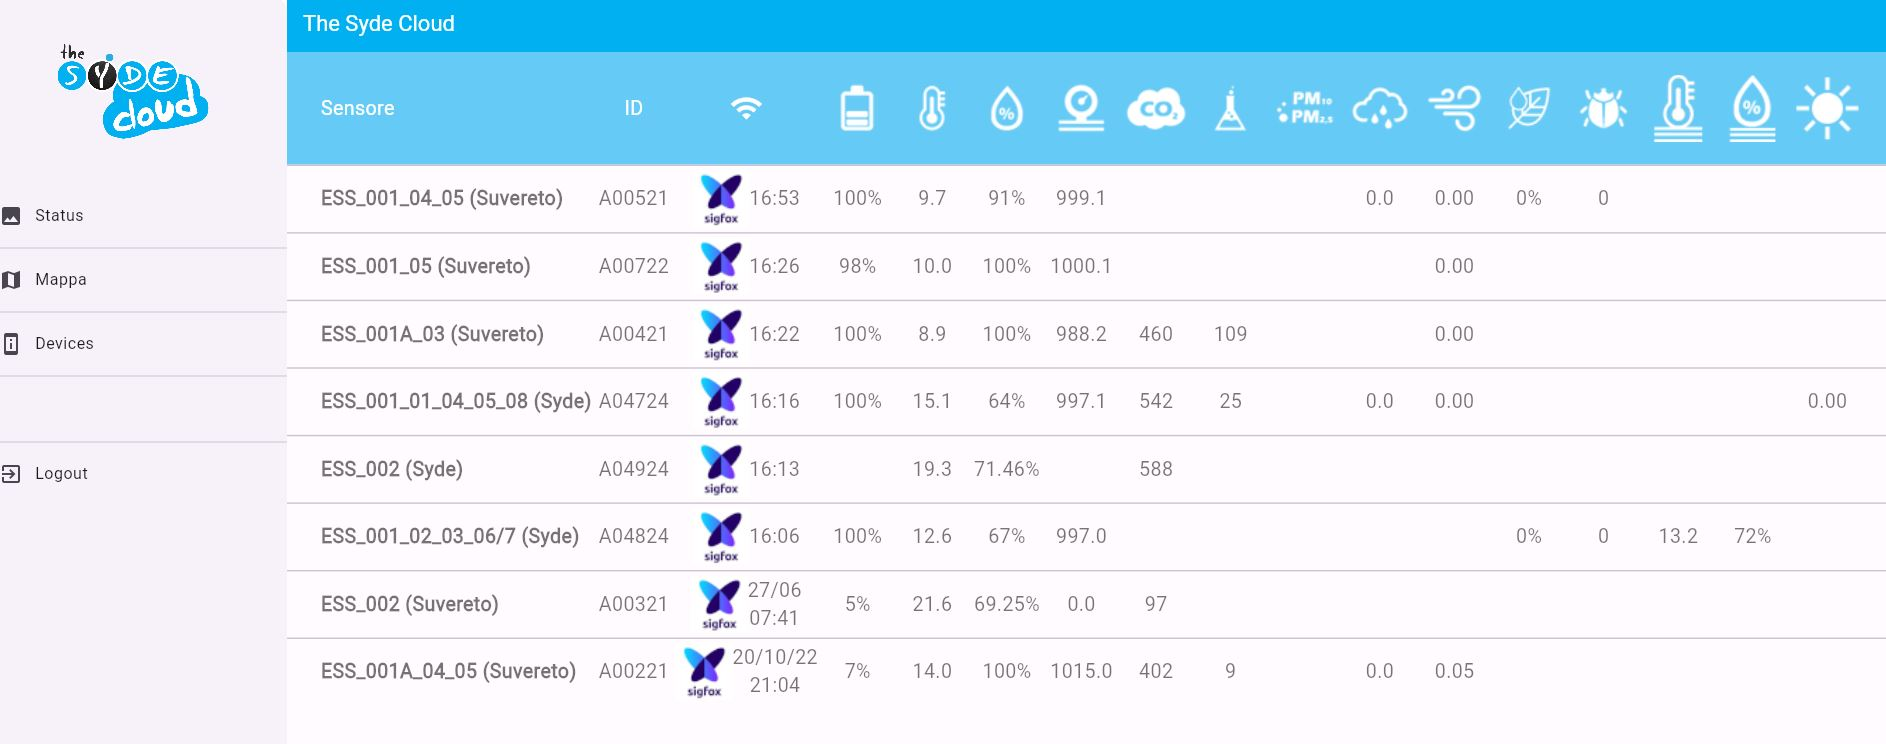
\includegraphics[trim=236.6mm 80mm 2.1mm 10mm, clip,scale=0.5]{../../Images/Syde/SydeCloud}


\bigskip

Description: Brightness



\bigskip

Unit: Watt per $m^2$


\bigskip

Minimum: 0 

\bigskip

Maximum: 100



\section{Download the Data}

The data can be downloaded via the command

\medskip
\URL{https://europe-west3-plasma-myth-295409.cloudfunctions.net/exportCSV?tkn=U3V2ZXJldG8=}

\medskip

or

\medskip

\URL{https://europe-west3-plasma-myth-295409.cloudfunctions.net/exportCSV?tkn=RmlyZW56ZQ== }


\medskip

These commands download a file named \FILE{sensori.csv}, which contains the actual sensor data values. 

\medskip

\textbf{Attention:} Both commands load a file named \FILE{sensori.csv}, but the contains is different. There are two set of sensors.

\medskip

{\tiny
\lstinputlisting{../../images/Syde/sensori.csv}
}

\bigskip

{\tiny
\lstinputlisting{../../images/Syde/sensori (1).csv}
}

